\documentclass[a4paper,12pt]{report}
\usepackage[utf8]{vietnam}
\usepackage{graphicx}
\usepackage{fancybox}
\usepackage{longtable}
\usepackage{listings}
\usepackage{relsize}
\usepackage[left=3cm, right=2.00cm, top=2.00cm, bottom=2.00cm]{geometry}
\lstset{
   %keywords={break,case,catch,continue,else,elseif,end,for,function,
   %   global,if,otherwise,persistent,return,switch,try,while},
   basicstyle=\ttfamily \fontsize{12}{15}\selectfont,   
	% numbers=left,
   frame=lrtb,
tabsize=2
}
\usepackage{hyperref}
\usepackage{float}
\hypersetup{
    colorlinks,
    citecolor=black,
    filecolor=black,
    linkcolor=black,
    urlcolor=black
}
\usepackage[nottoc]{tocbibind}
\usepackage[english]{babel}
\addto\captionsenglish{%
 \renewcommand\chaptername{Phần}
 \renewcommand{\contentsname}{Mục lục} 
 \renewcommand{\listtablename}{Danh sách bảng}
 \renewcommand{\listfigurename}{Danh sách hình vẽ}
 \renewcommand{\tablename}{Bảng}
 \renewcommand{\figurename}{Hình}
}
\begin{document}
\thispagestyle{empty}
\thisfancypage{
\setlength{\fboxrule}{1pt}
\doublebox}{}
\begin{center}
{\fontsize{16}{19}\fontfamily{cmr}\selectfont TRƯỜNG ĐẠI HỌC BÁCH KHOA HÀ NỘI\\
VIỆN CÔNG NGHỆ THÔNG TIN VÀ TRUYỀN THÔNG}\\
\textbf{------------*******---------------}\\[1cm]

\includegraphics[scale=0.13]{hust.jpg}\\[1.3cm]

{\fontsize{32}{43}\fontfamily{cmr}\selectfont BÁO CÁO}\\[0.1cm]
{\fontsize{38}{45}\fontfamily{cmr}\fontseries{b}\selectfont MÔN HỌC}\\[0.2cm]
{\fontsize{19}{20}\fontfamily{phv}\selectfont Học máy }\\[0.2cm]
{\fontsize{13}{20}\fontfamily{cmr}\selectfont Đề tài: So sánh thử nghiệm các phương pháp học máy\\ cho bài toán phân loại ảnh.
}\\[2.5cm]
\end{center}
\hspace{1cm}\fontsize{14}{16}\fontfamily{cmr}\selectfont \textbf{Nhóm sinh viên thực hiện:}

\begin{longtable}{l c c}

Họ và tên & MSSV  & Lớp\\
Nguyễn Tuấn Đạt & 20130856 & CNTT2.02-K58 \\
Vũ Minh Đức & 20130856 & CNTT2.02-K58 \\
Nguyễn Ngọc Huyền & 20130856 & CNTT2.02-K58 \\
Đặng Quang Trung & 20130856 & CNTT2.02-K58 \\
Phan Anh Tú & 20130856 & CNTT2.02-K58 \\

\end{longtable}

\hspace{1cm}\fontsize{14}{16}\fontfamily{cmr}\selectfont \textbf{Giáo viên hướng dẫn: }TS.Thân Quang Khoát \\[1.5cm]
\begin{center}
\fontsize{16}{19}\fontfamily{cmr}\selectfont Hà Nội 12--2016

\end{center}
\newpage
\pdfbookmark{\contentsname}{toc}
\tableofcontents
\chapter*{Lời cảm ơn}
\phantomsection
\addcontentsline{toc}{chapter}{Lời cảm ơn}

\listoffigures
\chapter{Mở đầu}
\chapter{Giới thiệu bài toán}
\section{Giới thiệu bài toán}
\section{Bộ dữ liệu sử dụng}
\chapter{Các phương pháp sử dụng và kết quả thực nghiệm}
\section{KNN}
\subsection{Cơ sở lý thuyết}
\subsection{Cài đặt}
(ghi chú: cần nêu rõ cấu trúc mã nguồn, chương trình, vai trò của các lớp và các phương thức chính)

\subsection{Kết quả}
\section{Mạng neural}
\section{Convolutional Neural Networks(CNN)}
\subsection{Giới thiệu}
Convolutional Neural Networks tương tư như các mạng nerual network khác. Chúng được tạo thành từ các tế bào noron có thể học trọng số và biases.Mỗi noron thực hiện hiện môt số sản xuất và tùy chọn với đường phi tuyến.Toàn bộ mạng vẫn thể hiện một hàm số khả vi duy nhất: từ các điểm ảnh hình ảnh thô trên một đầu với điểm số lớp học khác. Chúng vẫn có một hàm lỗi(ví dụ như SVM/softmax) ở lớp cuỗi (với kết nối đầy đủ).
\subsection{Kiến trúc tổng quan CNN}
Mạng CNN có 4 tầng chính: Convolution Layer, ReLu Layer , Pooling Layer, Fully-Connected Layer.
\subsubsection{Lớp Convolution Layer (Conv)}
\begin{itemize}
\item[-] Nhận đầu vào là ma trận các điểm ảnh $(W_1*H_1*D_1)$ ($W_1*H_1$: kích thước của ảnh, $D_1$ số kênh màu (3 kênh màu nếu là ảnh màu đại diện cho 3 kênh màu (r,g,b))).
\item[-] Các tham số:
\begin{itemize}
\item[•] Số các filters K: Tham số chính của tâng Conv. Mỗi filter sẽ trượt qua ma trận đầu vào và đưa ra ma trận đầu ra. Mỗi filter là một ma trận có kích thước là tham số cần chọn, chiều của ma trận là chiều của ma trận đầu vào (trong bài toán này chiều của filter là 3 (số kênh màu)).
\item[•] Kích thước của mỗi filter F*F.
\item[•] Số ô nhat qua mỗi lần trượt.
\item[•] Zerro padding P: Tham số quyết định ma trận đầu vào và ma trận đầu ra có cùng kích thước không (có trượt hết tất cả các ô của ma trận đầu vào không hay nói cách khác là có trượt vượt ra khỏi ma trận đầu vào không).
\end{itemize}
\item[-] Đầu ra là ma trận kích thước $W_2*H_2*D_2$:
\begin{itemize}
\item[•] $W_2 = (W_1 - F + 2P)/S + 1$.
\item[•] $H_2 = (H_1 - F + 2P)/S + 1$.
\item[•] $D_2 = K$.
\end{itemize}
\end{itemize}
\subsubsection{Lớp RELU Layer}
Tầng sẽ áp dụng hàm tác động, thông thường sẽ làm hàm ReLu max(0,x).Hàm sẽ tác động lên từng phần tử của ma trận đầu vào nên ma trận đi qua tầng này sẽ không thay đổi kích thước.
\subsubsection{Lớp PoolingLayer}
\begin{itemize}
\item[-] Thường chèn tầng pooling vào giữa các tầng Conv để giảm kích thước ma trận.
\item[-] Nhận đầu vào là ma trận $W_1*H_1*D_1$ là kích thước của ma trận đầu ra của tầng Conv.
\item[-] Các tham số:
\begin{itemize}
\item[•] Kích thước của ma trận pooling $F*F$.
\item[•] Số ô nhảy qua sau mỗi lần trượt trên ma trận input.
\end{itemize}
\item[-] Đầu ra là mậ trận kích thước $W_2*H_2*D_1$.
\begin{itemize}
\item[•] $W_2 = \frac{(W_1 - F)}{S} + 1$.
\item[•] $H_2 = \frac{(H_1 - F)}{S} + 1$.
\item[•] $D_2 = D_1$.
\end{itemize}
\end{itemize}
\subsubsection{Lớp Fully-connected Layer}
\begin{itemize}
\item[-] Như mạng neuron thông thường,các neuron trong tầng Fully-connected kết nối với toàn bộ các neuron ở tầng trước nó: Nhận đầu vào là vector áp dụng hàm tác động và đưa ra đầu ra.
\end{itemize}
\begin{figure}[h]
\begin{center}
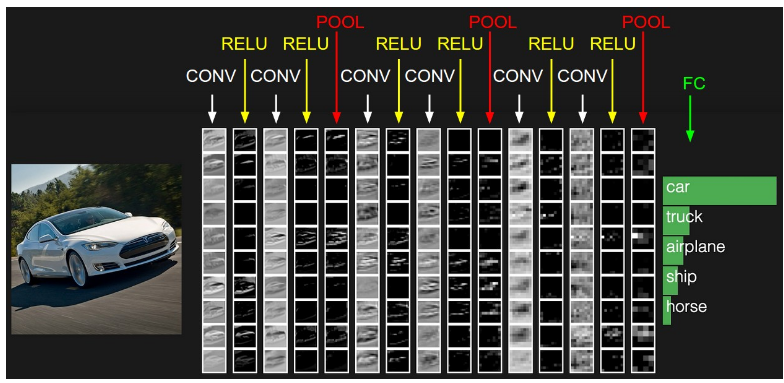
\includegraphics[width =0.8 \textwidth]{ConvNetArchitecture.png}
\end{center}
\end{figure}
\subsubsection{Lớp Max norm constraint và Dropout}
Để giảm overfit ta có thể áp dụng các kỹ thuật như:
\begin{itemize}
\item[-] Thêm max norm constraint cho các trọng số.
\begin{itemize}
\item[•] Khi cập nhật các trọng số thì các trường số phải thỏa mãn điều kiện: \\ 
 $\Vert\overrightarrow{w}\Vert_{2} < c$(c thường được chọn 3 hoặc 4). 
\end{itemize}
\item[-] Thêm tầng dropout
\begin{itemize}
\item[•] Đầu ra của các tầng trước tầng drop-out khi đi qua tầng drop-out sẽ được giữ nguyên với xác là p hoặc sẽ được chuyển thành 0 với xác suất 1-p.
\end{itemize} 
\end{itemize}
\subsection{Update tham số}
\subsubsection{Momentum update}
$\Delta w^{t+1} = \Delta w^{t} + \mu .\Delta w^{t} - \eta . \nabla E^t$.
\subsubsection{Nesterov momentum}
$w^{(t+1) = w^{t} + \mu . \Delta w^t}$ \\
$\Delta w^{(t+1)} = \mu . \Delta w^t - \eta . \nabla E^{t+1}$.
\begin{figure}[h]
\begin{center}
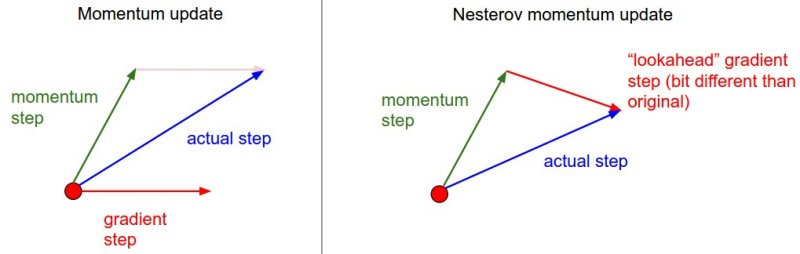
\includegraphics[width =0.8 \textwidth]{paramUpdate.jpeg}
\end{center}
\end{figure}
\subsection{Mạng CNN Đơn giản}
\subsubsection{Cấu trúc mạng}
\subsubsection{Cài đặt chương trình}
Sử dụng thư viện keras
\begin{itemize}
\item[-] Load data và xử lí dữ liệu:
\begin{figure}[h]
\begin{center}
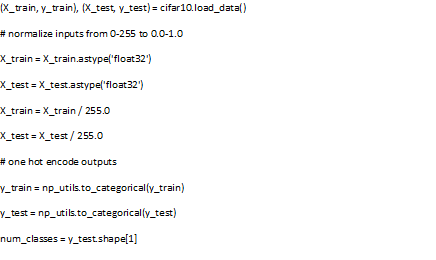
\includegraphics[width =0.7 \textwidth]{code1.png}
\end{center}
\end{figure}
\item[-] Thêm các tầng
\begin{figure}[h]
\begin{center}
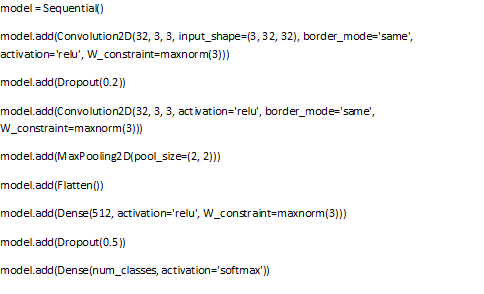
\includegraphics[width =0.7 \textwidth]{code2.png}
\end{center}
\end{figure}
\begin{itemize}
\item[•] Các tầng Conv có các tham số:
\begin{itemize}
\item[*] Số filter: 32
\item[*] Kích thước mỗi filter: $3*3*3$.
\item[*] input\_shape: Nhận đầu vào là ma trận ảnh $32*32*3$.
\item[*] border\_mode: kích thước ma trận đầu vào và ma trận đầu ra là như nhau (32*32).
\item[*] W\_constraint: max norm constraint với c = 3.
\end{itemize}
\item[•] Sau mỗi tầng Conv là tầng ReLu
\item[•] Tầng Drop-out thứ nhất với xác suất chuyển các tham số về 0 là 0.2
\item[•] Tầng Pooling với fiter có kích thước 2*2
\item[•] Tầng Flattern để chuyển ma trận thành vector 
\item[•] Tầng Dense (Fully-connected):
\begin{itemize}
\item[*] Kích thước đầu ra: 512 (vector 512 chiều)
\item[*] Hàm tác động: relu
\item[*] W\_constraint:  max norm constraint với c = 3
\end{itemize}
\item[•] Tầng Drop-out thứ hai với xác suất chuyển các tham số về 0 là 0.2
\item[•] Tầng Dense (Fully-connected) cuối cùng:
\begin{itemize}
\item[*] Kích thước đầu ra: Số nhãn lớp (scroce cho mỗi nhàn lớp): 10 nhãn lớp
\item[*] Hàm tác động : softmax (vector x có n chiều) \\ \\ 
\hspace*{2cm} $\sigma(x_i) = \frac{e^{x_i}}{\Sigma_{j=1}^{n}e^{x_k}}$
\end{itemize}
\end{itemize}
\item[-] Traning:
\begin{figure}[h]
\begin{center}
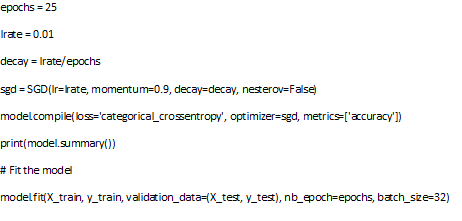
\includegraphics[width =0.7 \textwidth]{code3.png}
\end{center}
\end{figure}
\begin{itemize}
\item[•] Số epoch thực hiện 25
\item[•] Learning rate: 0.01
\item[•] Sử dụng minibatch gradient decent (số ảnh trong một batch là 32) với chiến lược tối ưu là momentum để update các tham số (tham số mu trong momentum là 0.9) không sử dụng nesterov momentum
\item[•] Hàm đánh giá lỗi: cross-entropy \\
\begin{center}
$L = -\frac{1}{N}\Sigma_{i=1}^{N}\big[y_i\log y_i + (1-\tilde{y_i})\big]$ (c là nhãn thực tế của ảnh i,$\tilde{y_i}$ là nhãn do mô hình dự đoán)
\end{center}
\end{itemize}
\end{itemize}
\subsubsection{Kết quả}
\begin{figure}[h]
\begin{center}
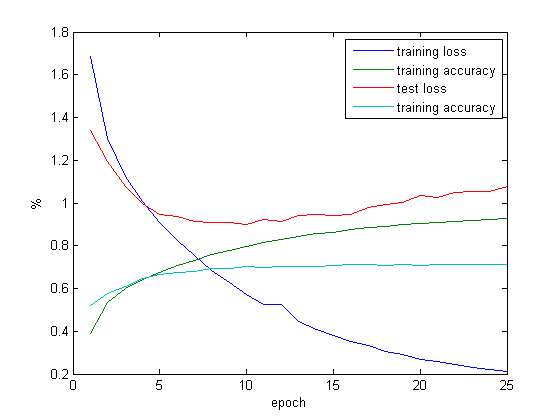
\includegraphics[width =1.0 \textwidth]{testImg.png}
\end{center}
\end{figure}
\subsection{Mạng CNN Lớn}
\subsubsection{Cấu trúc mạng}
{\small
$\textbf{INPUT} \rightarrow \textbf{CONV} \rightarrow \textbf{RELU} \rightarrow \textbf{DropOut} \rightarrow \big[\textbf{CONV} \rightarrow \textbf{RELU} \rightarrow \textbf{POOL\big]*2} \rightarrow \textbf{DropOut} \rightarrow \textbf{CONV} \rightarrow \textbf{RELU} \rightarrow \textbf{POOL} \rightarrow \textbf{FLatten} \big[\textbf{DropOut} \rightarrow \textbf{Fully-connect(RELU)\big]*2}\rightarrow \textbf{DropOut} \rightarrow \textbf{Ouput(num\_class,activation='softmax')}$
}
\newpage
{\small
\begin{center}
\begin{longtable}{lccl}
\caption{\textbf{Bảng mô tả mạng CNN}}
\label{variability_impl_mech}
\endfirsthead
\endhead
\hline
	Layer (type)              &      Output Shape     &     Param\#   &  Connected to  \\
\hline
convolution2d\_1 (Convolution2D) & (None, 32, 32, 32) &   896    &     convolution2d\_input\_1[0][0]     \\
\hline
dropout\_1 (Dropout)          &    (None, 32, 32, 32)  &  0     &      convolution2d\_1[0][0]            \\
\hline
convolution2d\_2 (Convolution2D)&  (None, 32, 32, 32) &   9248   &     dropout\_1[0][0]          \\        
\hline
maxpooling2d\_1 (MaxPooling2D)   & (None, 32, 16, 16)&    0       &    convolution2d\_2[0][0]      \\      
\hline
convolution2d\_3 (Convolution2D) & (None, 64, 16, 16) &   18496   &    maxpooling2d\_1[0][0] \\             
\hline
maxpooling2d\_2 (MaxPooling2D)   & (None, 64, 8, 8)    &  0        &   convolution2d\_3[0][0] \\
\hline
convolution2d\_4 (Convolution2D) & (None, 128, 8, 8)  &   73856   &    maxpooling2d\_2[0][0]      \\       
\hline
dropout\_2 (Dropout)  &            (None, 128, 8, 8) &    0   &        convolution2d\_4[0][0]       \\     

\hline
convolution2d\_5 (Convolution2D)&  (None, 128, 8, 8) &    147584 &     dropout\_2[0][0]            \\      

\hline
maxpooling2d\_3 (MaxPooling2D) &   (None, 128, 4, 4) &    0   &        convolution2d\_5[0][0]     \\       

\hline
flatten\_1 (Flatten)        &      (None, 2048) &         0    &       maxpooling2d\_3[0][0]    \\        

\hline
dropout\_3 (Dropout)    &          (None, 2048)  &        0   &        flatten\_1[0][0]    \\              

\hline
dense\_1 (Dense)      &            (None, 1024)     &     2098176   &  dropout\_3[0][0]    \\              

\hline
dropout\_4 (Dropout)  &            (None, 1024)  &        0  &         dense\_1[0][0]      \\              
\hline
dense\_2 (Dense)       &           (None, 512)  &         524800&      dropout\_4[0][0]        \\          

\hline
dropout\_5 (Dropout)    &          (None, 512) &          0      &     dense\_2[0][0]        \\           

\hline
dense\_3 (Dense)         &         (None, 10) &           5130    &    dropout\_5[0][0]          \\        

\hline
\end{longtable} 
\end{center}
}
Tổng params: 2878186
\section{SVM}
\chapter{Kết luận}
\section{So sánh các phương pháp}
\section{Khó khăn gặp phải}
\section{Kinh nghiệm rút ra được}
\chapter{Tài liệu tham khảo}
\begin{verbatim}
[+] https://

\end{verbatim}


\end{document}